\documentclass[twocolumn]{IEEEtran}
\usepackage{graphicx}
\usepackage[utf8x]{inputenc}
\usepackage{times}
\usepackage{amssymb,amsfonts}
\usepackage[tbtags]{amsmath}
\usepackage{cite}
\usepackage{slashbox}
\usepackage{pict2e}
\usepackage{float}
\usepackage[all]{xy}
\usepackage{graphics,graphicx,color,colortbl}
\usepackage{times}
\usepackage{subfigure}
\usepackage{wrapfig}
\usepackage{multicol}
\usepackage{cite}
\usepackage{url}
\usepackage[tbtags]{amsmath}
\usepackage{amsmath,amssymb,amsfonts,amsbsy}
\usepackage{bm}
\usepackage{algorithm}
\usepackage{algorithmic}
\usepackage[centerlast, small]{caption}
\usepackage[colorlinks=true, citecolor=blue, linkcolor=blue, urlcolor=blue,
breaklinks=true]{hyperref}


\begin{document}
\title{Introducción al uso del procesador LatticeMico32}
\author{David Ricardo Martínez Hernández Código: $261931$\\
	Juan Sebastian Roncancio Arevalo Código: $261585$}
\maketitle
\markboth{Universidad Nacional de Colombia}{}
\floatname{algorithm}{Algoritmo}
\begin{keywords}
 FPGA, LM32, Make, Verilog.
\end{keywords}
\begin{abstract}
Se realizo la instalación de todas las herramientas necesarias en el sistema operativo Linux, distribución Ubuntu, basandonos en la pagina principal de Linux En Caja para la instalación de dichas herramientas. Realizando todas las actividades propuestas en la guía de laboratorio, obteniendo todos los resultados de manera eficiente y completa.
\end{abstract}

\section{Objetivos}
\begin{itemize}
 \item Instalar las herramientas de compilación para el procesador LM32.
 \item Identificar las características básicas del procesador LM32.
 \item Realizar una aplicación con el procesador LM32.
\end{itemize}

\section{Introducción}
\noindent
El procesador \textbf{LatticeMico32} es un procesador \textit{softcore} lo que quiere decir que su implementación deja de ser física para poder ser implementada por completo con los recursos lógicos de las FPGAs, este procesador esta basado en una arquitectura RISC que es el acrónimo de ``\textbf{reduced instruction set computer}'' estos procesadores tienen las siguientes características:
\begin{itemize}
 \item Instrucciones de tamaño fijo y presentadas en un reducido numero de formatos.
 \item Solo las instrucciones de carga y almacenamiento acceden a la memoria de  datos.
\end{itemize}
\noindent
El objetivo de crear estos procesadores es promover el paralelismo y la  segmentación de instrucciones y reducir el acceso a la memoria. Este procesador provee la visibilidad y portabilidad esperada para ser un dispositivo de diseño de hardware libre\footnote{Tomado de \cite{page1}, 07 de Marzo de 2012}.

\section{Materiales}
\begin{itemize}
 \item Cable serial
 \item Computador con Sistema Operativo Linux Ubuntu
 \item FPGA
\end{itemize}

\section{Procedimiento}
\subsection{Proceso para sintetizar y compilar}
\noindent
Para sintetizar o simular se deben seguir los siguientes pasos:
\begin{enumerate}
 \item Ingresar a la consola y ubicarse en el directorio $SIE/SoftCore/lm32/logic/sakc$.
 \item Tener un archivo con extensión $.ram$ en el directorio firmware y se realiza el make correspondiente.
 \item Escribir en consola make syn (para sintetizar).
 \item Escribir en consola make sim (para simular).
 \item Escribir en consola make view (para ver los resultados de la simulación en gtkwave).
\end{enumerate}
\noindent
Este es el código que aparece en el archivo $log$ de la dirección $$SIE/SoftCore/lm32/logic/sakc/firmware/boot0-serial$$
\begin{verbatim}
lm32-elf-gcc -MMD -O2 -Wall -g -s
-fomit-frame-pointer -mbarrel-shift-enabled
-mmultiply-enabled -mdivide-enabled
-msign-extend-enabled -c crt0ram.S
echo "digital2 crt0ram.o"
digital2 crt0ram.o

lm32-elf-gcc -MMD -O2 -Wall -g -s
-fomit-frame-pointer -mbarrel-shift-enabled
-mmultiply-enabled -mdivide-enabled
-msign-extend-enabled -c main.c
echo "digital2 main.o"
digital2 main.o

lm32-elf-gcc -MMD -O2 -Wall -g -s
-fomit-frame-pointer -mbarrel-shift-enabled
-mmultiply-enabled -mdivide-enabled
-msign-extend-enabled -c soc-hw.c
echo "digital2 soc-hw.o" 
digital2 soc-hw.o

lm32-elf-ld -nostdlib -nodefaultlibs
-Tlinker.ld  -Map image.map -N -o 
image crt0ram.o main.o soc-hw.o
echo "digital2 image" 
digital2 image

lm32-elf-objdump -h -S image > image.lst
echo "digital2 image.lst" 
digital2 image.lst
lm32-elf-objcopy -j .text -j .rodata -j
.data -O srec image image.srec
echo "digital2 image.srec" 
digital2 image.srec
../../tools/srec2vram/srec2vram
   image.srec 0x00000000 0x1000 > image.ram
echo "digital2 image.ram" 
digital2 image.ram
make: <<image.ram>> está actualizado.
\end{verbatim}

\begin{figure}[H]
	\centering
		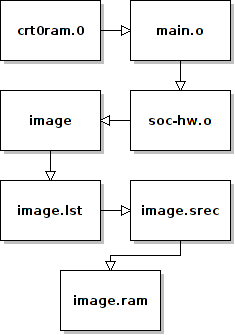
\includegraphics[scale=0.7]{UML.png}
	\caption{Diagrama de los pasos que realiza el archivo log}
	\label{fig1}
\end{figure}

\subsection{RTL y camino de datos}
\noindent
Se realizó el segundo procedimiento descrito en la guía de laboratorio para identificar la arquitectura del procesador LM32:
\begin{itemize}
 \item 
    \begin{enumerate}
     \item Ingresar a la consola en el directorio $SIE/SoftCore/lm32/logic/sakc/$
     \item Ingresar en la consola el comando \textbf{grep} de la siguiente forma:
\center{grep -IR RTL *}
    \end{enumerate}
\end{itemize}
\noindent
Salida desde consola de la carpeta $sack$ en consola el comando anterior:
\begin{verbatim}
123.txt:RTL Output                    
     : yes
123.txt:RTL Top Level Output File Name
     : system.ngr
build/system.ngc_xst.xrpt:        
<item stringID=
"XST_RTL_TOP_LEVEL_OUTPUT_FILE_NAME" 
value="system.ngr"/>
build/system.srp:RTL Output                     
     : yes
build/system.srp:RTL Top Level Output
 File Name
     : system.ngr
digital1.log:RTL Output                     
     : yes
digital1.log:RTL Top Level Output File Name
     : system.ngr
digital1.log:RTL Output                    
     : yes
digital1.log:RTL Top Level Output File Name
     : system.ngr
digital1.txt:RTL Output                     
     : yes
digital1.txt:RTL Output                  
     : yes
digital1.txt:RTL Top Level Output File Name
     : system.ngr
digital1.txt:RTL Output                    
     : yes
digital1.txt:RTL Top Level Output File Name
     : system.ngr
digital2.txt:RTL Output                    
     : yes
digital2.txt:RTL Top Level Output File Name
     : system.ngr
digi.txt:RTL Output                   
     : yes
laboratorio1/wb_sram32.syr:RTL Output      
     : Yes
laboratorio1/wb_sram32.syr:RTL Top Level
 Output File Name
     : wb_sram32.ngr
laboratorio1/wb_sram32_xst.xrpt:
<item stringID=
"XST_RTL_TOP_LEVEL_OUTPUT_FILE_NAME"
 value="wb_sram32.ngr"/>
laboratorio1/laboratorio1.restore:
"A" "" "" "" "PROP_xstGenerateRTLNetlist" "Yes" 
log:RTL Output                    
     : yes
log:RTL Top Level Output File Name
     : system.ngr
sim/ddr/readme.txt:To run simulations for this
sample configuration, user has to generate 
the RTL from the tool for the following GUI
\end{verbatim}
\begin{figure}[H]
	\centering
		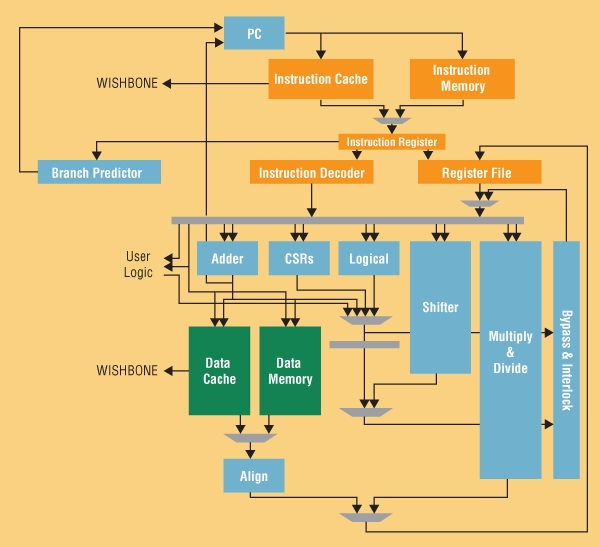
\includegraphics[scale=0.5]{RTL2_LM32.jpeg}
	\caption{Diagrama del RTL.(Tomado de \cite{page1})}
	\label{fig2}
\end{figure}
\begin{figure}[H]
	\centering
		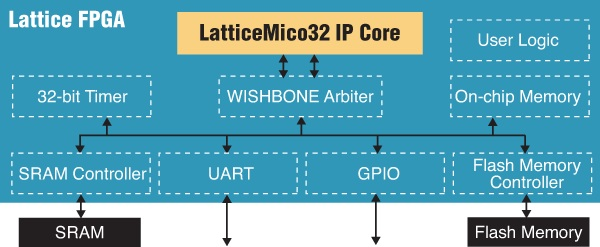
\includegraphics[scale=0.5]{RTL_LM32.jpeg}
	\caption{Diagrama del camino de datos (Datapath).(Tomado de \cite{page1})}
	\label{fig3}
\end{figure}
\noindent
Las instrucciones del  procesador $LM32$ son de $32$ bits y se encuentran  en cuatro formatos básicos que se listan a continuación:
\begin{table}[H]
	\centering
\begin{tabular}[c]{|c|c|c|c|c|} \hline
\textbf{1-bit} & \textbf{5-bit} & \textbf{5-bit} & \textbf{5-bit} & \textbf{16-bits} \\ \hline
0 & Opcode & Reg 0 & Reg 1 & Immediate \\ \hline
\end{tabular}
	\caption{Formato Inmediato}
	\label{tab1}
\end{table}
\begin{table}[H]
	\centering
\begin{tabular}[c]{|c|c|c|c|c|c|} \hline
\textbf{1-bit} & \textbf{5-bit} & \textbf{5-bit} & \textbf{5-bit} & \textbf{5-bit} & \textbf{11-bits} \\ \hline
1 & Opcode & Reg 0 & Reg 1 & Reg 2 & $1${$1$'b$0$} \\ \hline
\end{tabular}
	\caption{Formato Registro Registro}
	\label{tab2}
\end{table}
\begin{table}[H]
	\centering
\begin{tabular}[c]{|c|c|c|c|c|} \hline
\textbf{1-bit} & \textbf{5-bit} & \textbf{5-bit} & \textbf{5-bit} & \textbf{16-bits} \\ \hline
1 & Opcode & CSR 0 & Reg & $16${$1$'b$0$} \\ \hline
\end{tabular}
	\caption{Registro de Control}
	\label{tab3}
\end{table}
\begin{table}[H]
	\centering
\begin{tabular}[c]{|c|c|} \hline
\textbf{6-bit Register} & \textbf{26-bit Immediate} \\ \hline
$11100$(/$11$)$0$ & Immediate \\ \hline
\end{tabular}
	\caption{Formato Inmediato}
	\label{tab4}
\end{table}
\noindent
Algunas de las características clave de este procesador de 32-bits incluyen
\begin{itemize}
 \item RISC architecture
 \item $32$-bit data path
 \item $32$-bit instructions
 \item $32$ general-purpose registers
 \item Up to $32$ external interrupts
 \item Optional instruction cache
 \item Optional data cache
 \item Dual WISHBONE memory interfaces (instruction and data)
\end{itemize}
\noindent
Para acelerar el desarrollo de procesos del  procesador, se pueden adicionar  componentes periféricos. Específicamente, estos componentes están conectados al procesador a través de un WISHBONE interfaz de bus. Por utilizar este interfaz de origen de bus abierto, puede incorporar los componentes de Wishbone propias en los diseños embebidos. Los componentes incluyen:
\begin{itemize}
 \item Memory controllers
 \item Asynchronous SRAM
 \item Double data rate (DDR)
 \item On-chip
 \item Input/output (I/O) ports
 \item 32-bit timer
 \item Direct memory access (DMA) controller
 \item General-purpose I/O (GPIO)
 \item I2C master controller
 \item Serial peripheral interface (SPI)
 \item Universal asynchronous receiver transmitter (UART)
\end{itemize}
\begin{figure}[H]
	\centering
		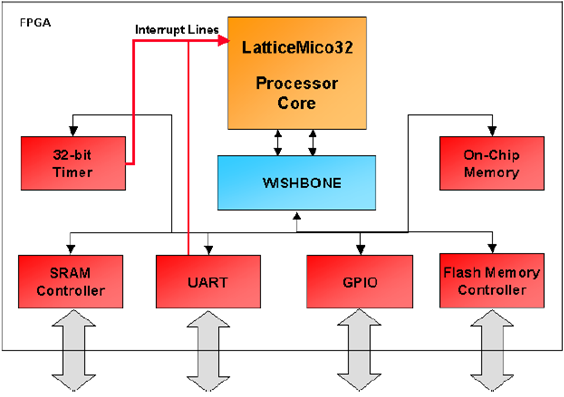
\includegraphics[scale=0.7]{fpga.png}
	\caption{Sistema completo utilizando el procesador junto con varios componentes}
	\label{fig4}
\end{figure}

\section{Aplicación}
\noindent
Este es el código utilizado para la aplicación de sumar $2$ números, es decir el \textit{main.c} y también se muestra la simulación del programa tomando como ejemplo $1+1$ fig. \ref{fig4}
\begin{verbatim}
#include "soc-hw.h"
/*prototypes */
uint32_t read_uint32()
{
	uint32_t val = 0, i;
    for (i = 0; i < 4; i++) {
        val <<= 8;
        val += (uint8_t)uart_getchar();
    }
    return val;
}

int main(int argc, char **argv)
{
	// Initialize UART
	uart_init();
	
	char a,b,c;
	a= uart_getchar();
	b= uart_getchar();
	c= a+b;
	uart_putchar(c);
}
\end{verbatim}

\begin{figure}[H]
	\centering
		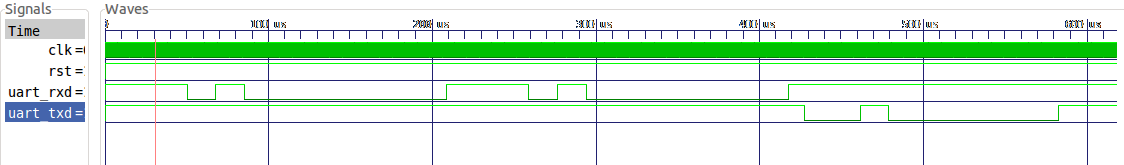
\includegraphics[scale=0.25]{sim.png}
	\caption{Simulación}
	\label{fig4}
\end{figure}

\section{Conclusiones}
\begin{itemize}
 \item Debido a la disponibilidad de los componentes de software libre, estos procesadores son y serán los pilares del desarrollo futuro, ya que por su bajo costo y su fácil implementación son las herramientas perfectas para el desarrollo de muchos dispositivos.
 \item Debido al escaso conocimiento sobre el sistema operativo basado en Linux nos tomo más tiempo del necesario instalar los componentes en dicho sistema operativo ya que  es un poco diferente a lo que estamos  acostumbrados a instalar en Windows, por lo tanto tuvimos que aprender a manejar comandos para usar la consola del sistema operativo basado en Linux. Y por esta razón el desarrollo de la practica estuvo un poco sesgada a la disponibilidad de los programas instalados en el sistema operativo.
\end{itemize}

\bibliographystyle{ieeetran}
\begin{thebibliography}{99}
\bibitem{patterson} Patterson, David \& Hennessy John
{\em "`Computer Organization And Design - The Hardware-Software Interface"'}.
Kindle Edition, Fourth Edition, 2006.

\bibitem{page1} \url{http://www.latticesemi.com/products/intellectualproperty/ipcores/mico32/index.cfm}

\bibitem{page1} \url{http://www.ohwr.org/documents/68}

\bibitem{page1} \url{http://www.linuxencaja.net/wiki/Arquitectura_LM32_JPRR_%28261744%29}
\end{thebibliography}
\end{document}